\documentclass[10pt,a4paper,twocolumn]{ctexart}
\usepackage[margin=15.5mm,top=15mm,bottom=17mm,columnsep=5.5mm]{geometry}
\usepackage{amsmath,amssymb,bm}
\usepackage{booktabs,multirow,tabularx}
\usepackage{graphicx}
\usepackage{microtype}
\usepackage{enumitem}
\usepackage{xcolor}
\usepackage{hyperref}
\usepackage{tikz}
\usetikzlibrary{arrows.meta,positioning,fit,calc,shapes.geometric,backgrounds}
\usepackage{algorithm}
\usepackage{algpseudocode}
\usepackage{caption}
\usepackage{subcaption}
\usepackage{balance}
\usepackage{fancyhdr}
\usepackage{pifont}
\usepackage{array}
\usepackage{ragged2e}

\definecolor{cblue}{RGB}{49,103,190}
\definecolor{cgreen}{RGB}{61,148,96}
\definecolor{corange}{RGB}{223,137,42}
\definecolor{cpurple}{RGB}{128,84,174}
\definecolor{clight}{RGB}{245,247,250}
\definecolor{cred}{RGB}{190,66,66}

\hypersetup{colorlinks=true,linkcolor=cblue,citecolor=cblue,urlcolor=cblue}
\captionsetup{font=small,labelfont=bf}
\setlength{\parindent}{1em}
\setlength{\parskip}{0pt}
\setlist[itemize]{leftmargin=1.3em,itemsep=1pt,topsep=2pt}
\setlist[enumerate]{leftmargin=1.5em,itemsep=1pt,topsep=2pt}
\pagestyle{fancy}
\fancyhf{}
\lhead{EvoRS-Comm: Hierarchical Multimodal Communication for Remote-Sensing Multi-Agent Systems}
\rhead{Draft}
\cfoot{\thepage}
\renewcommand{\headrulewidth}{0.25pt}

\title{\textbf{EvoRS-Comm：面向遥感视觉理解的自然演化多智能体框架\\——层次化多模态通信与结构化多智能体强化学习}}
\author{Anonymous Authors}
\date{}

\newcommand{\ours}{\textsc{EvoRS-Comm}}
\newcommand{\tree}{\mathcal{T}}
\newcommand{\msg}{\mathcal{M}}
\newcommand{\agentset}{\mathcal{A}}
\newcommand{\todo}{\textcolor{cred}{\textbf{TBD}}}

\begin{document}
\maketitle
\vspace{-1.4em}

\begin{abstract}
现有遥感视觉语言多智能体系统大多沿用通用 Agent 的文本通信范式：每个 Agent 将局部视觉理解压缩为自然语言，再由其他 Agent 基于文本继续推理。该过程虽然易于实现，但会丢失空间层次、精确位置与细粒度视觉证据；与此同时，现有多智能体强化学习通常将 Agent 输出视为同质文本 action，难以对遥感任务中的结构化空间消息与连续视觉表征进行联合优化。本文提出 \ours，一个面向遥感视觉理解的自然演化多智能体框架。其宏观目标是让 Agent 的职责、通信对象与通信载荷在任务训练中自适应形成，而不是完全依赖人工固定工作流。具体而言，我们提出层次化多模态通信协议，将遥感场景显式组织为 Scene--Region--Group--Object 四级共享树，并允许 Agent 同时交换文本消息、结构化节点/子树和图像 latent representation。进一步地，我们在 cooperative MARL 基础上提出结构化通信优化目标，将 ``给谁发、发哪个空间层级、使用何种模态、携带哪些节点/latent'' 纳入联合策略，并显式建模通信成本、结构一致性与消息冗余。本文给出完整的问题形式化、算法框架和实验协议；由于实验尚未执行，所有数值结果均以 \todo 标记，本文不预设任何性能提升。
\end{abstract}

\section{引言}
遥感图像与普通自然图像的一个重要差异在于其空间组织方式。遥感影像通常覆盖大范围地表区域，包含大量小目标、功能区域与重复结构。近年来的 VRSBench、XLRS-Bench、CHOICE 与 GEOBench-VLM 等 benchmark 已将遥感理解从单一分类扩展到 VQA、grounding、目标计数、空间关系、超高分辨率理解与时序分析等任务~\cite{vrsbench,xlrs,choice,geobench}。然而，现有多 Agent 视觉推理仍主要通过自然语言串联：一个 Agent 观察图像后输出文本，另一个 Agent 再从文本恢复语义与空间线索。

这种通信方式存在两个问题。第一，文本会将原本二维、层次化的视觉证据序列化。例如 ``图中存在五架飞机'' 并不能直接告诉接收方五个目标分别位于何处、属于哪个机坪区域、来自哪个 crop、哪些目标仍未验证。第二，图像 latent 与结构关系被压缩为离散 token 后难以无损恢复。最新的 latent agent communication 工作已经指出，纯文本通信会造成信息损失与额外推理开销，并开始直接交换 hidden state 或压缩 latent~\cite{interlat,macf}。但这些方法并未针对遥感场景的显式空间层次设计通信协议。

另一方面，遥感 Scene Graph 已从静态对象关系扩展到层次化和多尺度表示~\cite{knyaz2025,knyaz2026}；SG2 进一步表明多 Agent 可以对 scene graph 进行按需查询~\cite{sg2}。但这些工作主要将图视为视觉表示或检索对象，而不是一种贯穿多 Agent 强化学习过程的\textbf{共享通信状态}。本文关注的问题因此不是 ``能否生成遥感 scene graph''，而是：

\begin{quote}\small
\textbf{能否把遥感空间层次直接变成 Agent 的通信协议，并让 cooperative RL 学习何时传文本、何时传结构、何时直接传视觉 latent？}
\end{quote}

我们提出 \ours。其核心不是单独增加一个树结构，而是将 Agent communication action 从单一文本消息扩展为多维决策：
\begin{equation}
 a^{\mathrm{comm}}_t=
 (r_t,\ell_t,m_t,p_t),
 \label{eq:commaction}
\end{equation}
其中 $r_t$ 为接收 Agent，$\ell_t$ 为 Scene/Region/Group/Object 空间层级，$m_t$ 为 Text/Structure/Latent 通信模态，$p_t$ 为具体 payload。共享状态则由问题、层次树、Agent 历史与通信预算共同组成。随着训练进行，不同 Agent 可以在不同任务中形成不同的责任分工与通信模式，我们将这一现象称为\textbf{自然演化协作（natural-evolving collaboration）}；它指 policy-driven specialization，而非遗传算法意义上的 mutation/crossover。

\paragraph{本文贡献。}
\begin{enumerate}
    \item \textbf{自然演化遥感多 Agent 框架。} 提出以共享遥感空间状态为交互媒介的宏观框架，使 Agent 的合作对象、职责与消息形态能够随任务通过强化学习自适应演化，而非依赖单一 Router 或固定工作流。
    \item \textbf{多 Agent 分层多模态通信。} 将遥感图像显式组织为 Scene--Region--Group--Object 四级树，并设计 Text--Structure--Visual Latent 三通道消息，使语义、空间地址与原始视觉证据可以在 Agent 间联合传递。
    \item \textbf{结构化通信 MARL 算法。} 在 cooperative MARL/MAGRPO 思路上扩展 communication action space 与优化目标，同时学习 recipient、hierarchy level、message modality 和 payload，并加入结构一致性、通信成本与冗余抑制奖励。
    \item \textbf{系统性实验验证。} 设计覆盖 VRSBench、CHOICE、XLRS-Bench 与 GEOBench-VLM 的评测，包括准确率、跨任务泛化、通信 token、latent bandwidth 与通信效率。由于实验尚未执行，本文所有结果均为 \todo，不声明未验证的性能优势。
\end{enumerate}

\section{相关工作}
\subsection{遥感层次场景表示}
Knyaz 等研究了航拍图的层次 scene graph 与向量化，将对象关系与层级纳入遥感场景理解~\cite{knyaz2025}；后续工作进一步研究多尺度 scene graph generation~\cite{knyaz2026}。这些工作证明了 ``Scene--Region--Object'' 结构对于遥感视觉具有合理性，但主要目标仍是构建或评估 scene graph，而非将其变成多 Agent 的通信协议。本文不主张层次 scene graph 本身的新颖性，而是将其改造成可被 Agent 读写、按层级传递、挂接 visual latent 的共享通信状态。

\subsection{Scene Graph 与多 Agent 推理}
SG2 将 Reasoner 与 Retriever 分离，使多个 LLM Agent 通过 schema-guided query 从 scene graph 中迭代取数，避免一次注入完整图~\cite{sg2}。SaGe 则将 scene graph thinking 用于多模态结构化推理，并进一步采用 graph-aware post-training~\cite{sage}。与之不同，我们关注的是通信本身：结构树不仅是被查询的数据源，而是 Agent 消息的显式载体；同时，视觉 latent 与自然语言和结构节点一起进入 communication action space。

\subsection{多 Agent 强化学习与 latent communication}
MAGRPO 将 LLM collaboration 建模为 cooperative MARL，并通过 multi-agent group-relative policy optimization 联合优化多 Agent 策略~\cite{magrpo}。本文以此类方法为训练基础，但将通信动作从文本 response 扩展为层次化多模态消息。与此同时，Interlat 已验证 Agent 可以直接交换连续 hidden states，并报告了显著的推理加速潜力~\cite{interlat}；MACF 在长视频理解中使用 compact latent tokens 支持多 Agent 协作~\cite{macf}。这些结果说明视觉/语言 latent communication 在技术上可行。我们的重点是将 latent 明确绑定到遥感树节点及其 bbox/region，使连续表示具有可定位、可追溯的空间语义。

\section{问题定义}
给定遥感图像 $I$ 与问题 $q$，系统包含固定基础能力 Agent 集合
\begin{equation}
\agentset_F=\{A_G,A_L,A_H,A_V\},
\end{equation}
分别表示 Global、Local、Hierarchy 与 Verifier Agent；另设一个没有预定义细粒度职责的残差 Agent $A_E$。完整 Agent 池为
\begin{equation}
\agentset=\agentset_F\cup\{A_E\}.
\end{equation}
所有 Agent 共享同一遥感空间树 $\tree_t$，但可拥有独立 LoRA/adapter 与局部 observation。

系统在每轮 $t$ 维护共享状态
\begin{equation}
S_t=(q,\tree_t,H_t,B_t),
\end{equation}
其中 $H_t$ 为团队交互历史，$B_t$ 为剩余 token、image query、latent bandwidth 等预算。策略输出两类 action：任务动作 $a^{task}$ 与通信动作 $a^{comm}$。目标是在任务正确率与通信/视觉成本之间取得最优权衡。

\section{方法}
\subsection{总体框架：自然演化协作}
\begin{figure*}[t]
\centering
\resizebox{0.97\textwidth}{!}{%
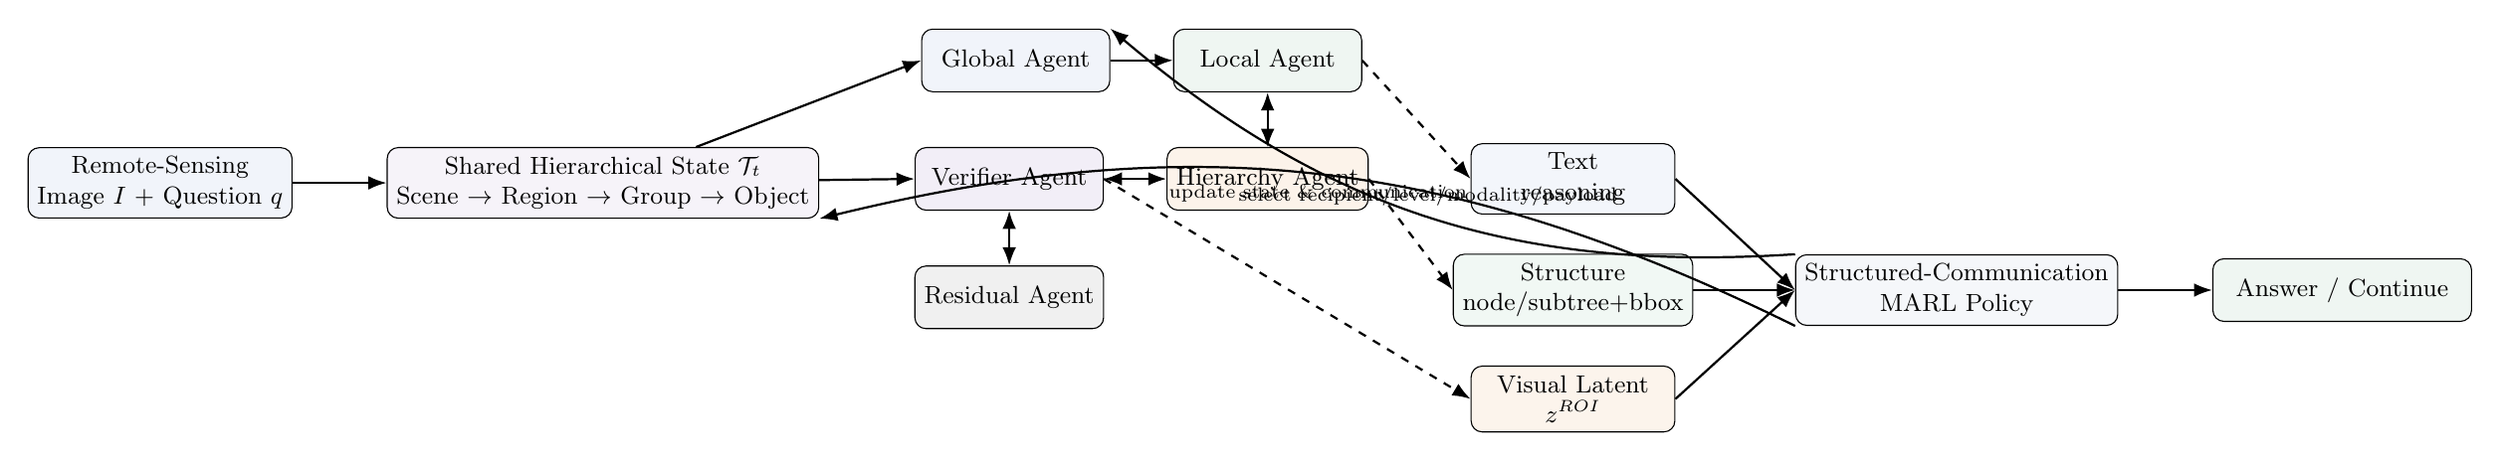
\begin{tikzpicture}[font=\small,>=Latex,node distance=5mm and 7mm,
box/.style={rounded corners,draw,minimum height=8mm,align=center,fill=white},
agent/.style={box,minimum width=24mm},
state/.style={box,fill=clight,minimum width=33mm},
msg/.style={box,minimum width=26mm},
arr/.style={->,thick}]
\node[state,fill=cblue!7] (input) {Remote-Sensing\\Image $I$ + Question $q$};
\node[state,right=12mm of input,fill=cpurple!7] (tree) {Shared Hierarchical State $\tree_t$\\Scene $\rightarrow$ Region $\rightarrow$ Group $\rightarrow$ Object};
\node[agent,above right=7mm and 13mm of tree,fill=cblue!7] (g) {Global Agent};
\node[agent,right=8mm of g,fill=cgreen!8] (l) {Local Agent};
\node[agent,below=7mm of l,fill=corange!10] (h) {Hierarchy Agent};
\node[agent,left=8mm of h,fill=cpurple!10] (v) {Verifier Agent};
\node[agent,below=7mm of v,fill=gray!12] (e) {Residual Agent};
\node[msg,right=13mm of h,fill=cblue!6] (text) {Text\\reasoning};
\node[msg,below=5mm of text,fill=cgreen!7] (struct) {Structure\\node/subtree+bbox};
\node[msg,below=5mm of struct,fill=corange!9] (latent) {Visual Latent\\$z^{ROI}$};
\node[state,right=13mm of struct,fill=clight] (policy) {Structured-Communication\\MARL Policy};
\node[state,right=12mm of policy,fill=cgreen!8] (ans) {Answer / Continue};
\draw[arr] (input)--(tree);
\draw[arr] (tree)--(g.west);
\draw[arr] (tree)--(v.west);
\draw[arr] (g)--(l);
\draw[arr,<->] (l)--(h);
\draw[arr,<->] (h)--(v);
\draw[arr,<->] (v)--(e);
\draw[arr,dashed] (l.east)--(text.west);
\draw[arr,dashed] (h.east)--(struct.west);
\draw[arr,dashed] (v.east)--(latent.west);
\draw[arr] (text.east)--(policy.west);
\draw[arr] (struct.east)--(policy.west);
\draw[arr] (latent.east)--(policy.west);
\draw[arr] (policy)--(ans);
\draw[arr,bend left=22] (policy.north west) to node[above,font=\scriptsize]{select recipient/level/modality/payload} (g.north east);
\draw[arr,bend right=20] (policy.south west) to node[below,font=\scriptsize]{update state \& communication} (tree.south east);
\end{tikzpicture}%
}
\caption{\ours 总体框架。共享遥感层次状态作为所有 Agent 的显式空间通信骨架。通信不仅包含文本，还可以传递结构化节点/子树以及与节点绑定的视觉 latent。强化学习策略联合决定接收方、空间层级、消息模态和 payload，使协作模式在任务训练中自适应形成。}
\label{fig:overview}
\end{figure*}

我们将 ``自然演化'' 定义为从固定初始 Agent 能力出发，在训练中由 policy 逐渐形成任务依赖的通信拓扑与责任分配。系统不要求所有 Agent 每题都参与，也不预先固定 ``计数专家''、``机场专家'' 等细粒度角色。基础专家只提供少量遥感先验能力，而 $A_E$ 用于吸收固定角色未覆盖的残差行为。

\subsection{四级遥感共享状态}
我们使用四级树表示空间层次：
\begin{equation}
\tree_t: \mathrm{Scene}\rightarrow\mathrm{Region}\rightarrow\mathrm{Group}\rightarrow\mathrm{Object}.
\end{equation}
每个节点 $v_i$ 定义为
\begin{equation}
 v_i=(id_i,\ell_i,s_i,b_i,c_i,u_i,z_i,p_i),
 \label{eq:node}
\end{equation}
其中 $\ell_i$ 为层级，$s_i$ 为语义标签，$b_i$ 为 bbox/polygon，$c_i$ 为 confidence，$u_i$ 为 uncertainty，$z_i$ 为可选 visual latent，$p_i$ 为 evidence provenance。一个机场场景可表示为
\[
\mathrm{Airport}\rightarrow\mathrm{Apron}\rightarrow\mathrm{AircraftGroup}\rightarrow\mathrm{Aircraft}_k.
\]
与自然语言相比，该状态显式保留 ``谁属于谁'' 以及 ``目标在哪里''，因此接收 Agent 可以直接使用 $b_i$ 调用 crop/zoom/detector 等视觉工具。

\begin{figure*}[t]
\centering
\includegraphics[width=0.98\textwidth]{figures/refinement.png}
\caption{概念性示例：问题驱动的层次细化过程。共享树可以从 Scene 逐步定位到 Region、Group 与 Object，最终把回答所需的对象位置和数量显式交给下游 Agent。图中影像与示意布局用于方法说明，不代表实验结果。}
\label{fig:refine}
\end{figure*}

\subsection{层次化多模态通信协议}
传统 Agent 消息通常只有文本 $M^{text}$。我们将消息扩展为
\begin{equation}
M_{i\rightarrow j}=\big(M^{text},M^{struct},M^{latent}\big),
\label{eq:message}
\end{equation}
但每次通信无需发送全部三种模态，而是由策略按需选择。

\paragraph{Text channel.} 用于自然语言推理、任务意图和高层解释。例如 ``当前区域可能为机场，但需要验证机坪中的小目标''。

\paragraph{Structured channel.} 直接发送一个节点、路径或子树，例如
\[
\{\mathrm{Apron},\mathrm{AircraftGroup},b_{ROI},c,u\}.
\]
结构消息承担\textbf{空间地址与语义骨架}功能，下游 Agent 不必从文本重新恢复 bbox 与层次关系。

\paragraph{Visual latent channel.} 对某个节点对应区域 $I[b_i]$，视觉编码器产生
\begin{equation}
 z_i=C_\omega\left(E_{vis}(I[b_i])\right)\in\mathbb{R}^{K\times d},
 \label{eq:latent}
\end{equation}
其中 $C_\omega$ 是可学习压缩器。如果所有 Agent 共享 backbone，则 $z_i$ 可直接复用；若 Agent 异构，则采用投影器 $P_{i\to j}$ 对齐 latent space。接收 Agent 通过 cross-attention 融合：
\begin{equation}
\tilde h_j=h_j+\mathrm{Attn}(h_j,P_{i\to j}z_i,P_{i\to j}z_i).
\end{equation}
因此 Tree 负责 ``这是什么、在哪里''，latent 负责 ``它具体长什么样''，text 负责 ``为什么发送它、下一步推理目的是什么''。

\subsection{通信决策空间}
在每个 step，通信策略不只选择 next agent，而是选择
\begin{equation}
a_t^{comm}=(r_t,\ell_t,m_t,p_t),
\end{equation}
其中
\begin{align*}
 r_t &\in \agentset,\\
 \ell_t &\in \{scene,region,group,object\},\\
 m_t &\in \{text,struct,latent,hybrid\},\\
 p_t &\subseteq \tree_t.
\end{align*}
``hybrid'' 可以是 Text+Struct、Struct+Latent 或三者联合。该设计使通信选择本身成为可优化 action：简单高层任务可只传短文本或场景节点；小目标复核可传 Object node + latent；复杂空间关系则传子树。

\subsection{结构化通信多智能体强化学习}
MAGRPO 已证明可以用 group-relative objective 优化 LLM multi-agent collaboration~\cite{magrpo}。我们在此基础上将每个 Agent 的 policy 拆为 task policy 与 communication policy：
\begin{equation}
\pi_i(a_t|o_i,S_t)=\pi_i^{task}(a_t^{task}|\cdot)\,\pi_i^{comm}(a_t^{comm}|\cdot).
\end{equation}
团队奖励设计为
\begin{equation}
R=R_{task}+\lambda_s R_{struct}+\lambda_e R_{evid}-\lambda_c C_{comm}-\lambda_r C_{red}.
\label{eq:reward}
\end{equation}
其中 $R_{task}$ 为最终答案奖励；$R_{struct}$ 衡量树结构一致性；$R_{evid}$ 鼓励消息可追溯到视觉证据；$C_{comm}$ 为通信成本；$C_{red}$ 惩罚重复消息。

通信成本按不同模态分别计量：
\begin{equation}
C_{comm}=\alpha N_{text}+\beta N_{node}+\gamma N_{latent},
\end{equation}
使策略在 ``信息充分'' 与 ``带宽开销'' 之间学习折中。

为避免所有 Agent 重复传递相同结论，我们定义消息新颖性辅助奖励：
\begin{equation}
r^{novel}(m_t)=1-\max_{m\in H_t}\mathrm{sim}(m_t,m),
\end{equation}
并将其与 evidence gain 结合得到局部 communication reward
\begin{equation}
r_t^{comm}=\eta_1\Delta E_t+\eta_2r^{novel}(m_t)-\eta_3 cost(m_t).
\end{equation}

在 group-relative advantage $\hat A^{team}$ 的基础上，通信分支使用
\begin{equation}
\hat A_t^{comm}=\hat A^{team}+\rho\,\mathrm{norm}(r_t^{comm}),
\end{equation}
从而让 ``答对但通信极其冗余'' 与 ``答对且通信有效'' 的轨迹获得不同 credit。

最终优化目标采用两套 clipping：
\begin{equation}
\resizebox{0.98\columnwidth}{!}{$\displaystyle
\mathcal{L}_{HM\text{-}MAGRPO}=\mathbb{E}\!\left[
\min(r_t^{task}\hat A^{team},\mathrm{clip}(r_t^{task},1\!\pm\!\epsilon_t)\hat A^{team})
+\kappa\min(r_t^{comm}\hat A_t^{comm},\mathrm{clip}(r_t^{comm},1\!\pm\!\epsilon_c)\hat A_t^{comm})
\right]$}
\label{eq:hmgrpo}
\end{equation}
其中 $r_t^{task}$ 和 $r_t^{comm}$ 分别为新旧策略概率比。式~\eqref{eq:hmgrpo} 是本文相对 generic MAGRPO 的核心算法改动：通信不再被隐含在文本 generation 中，而是作为独立、结构化、可计成本的策略分支进行优化。

\begin{algorithm}[t]
\caption{HM-MAGRPO 训练流程（简化）}
\label{alg:train}
\begin{algorithmic}[1]
\Require dataset $\mathcal D$, agent pool $\agentset$, initial policies $\pi$
\For{each training batch $(I,q,y)$}
  \State 初始化共享树 $\tree_0$ 与预算 $B_0$
  \For{$t=0,\ldots,T-1$}
    \State 各 active Agent 读取 $S_t=(q,\tree_t,H_t,B_t)$
    \State 采样 task action 与 $a_t^{comm}=(r,\ell,m,p)$
    \State 发送 Text/Structure/Latent 消息并更新 $\tree_{t+1}$
    \If{stop or answer} \State \textbf{break} \EndIf
  \EndFor
  \State 计算 $R_{task},R_{struct},R_{evid},C_{comm},C_{red}$
  \State 对同一问题的 group trajectories 计算 $\hat A^{team}$
  \State 计算 $\hat A^{comm}$ 并更新 task/communication policies
\EndFor
\end{algorithmic}
\end{algorithm}

\subsection{跨层结构一致性与证据追溯}
树中高层结论必须能被低层节点支持。例如 Aircraft 应属于 AircraftGroup，AircraftGroup 属于 Apron，而 Apron 属于 Airport。若不同 Agent 写入的结构产生冲突，Verifier 可沿 provenance 定位到具体节点和 ROI，再调用视觉工具重新验证。

\begin{figure}[t]
\centering
\includegraphics[width=\columnwidth]{figures/crossscale.png}
\caption{跨层结构一致性示意。高层 Scene/Region 语义与中层 Group、细粒度 Object 证据发生冲突时，系统触发 revise/refine，而不是仅在文本层做多数投票。}
\label{fig:consistency}
\end{figure}

\section{实验设计}
\subsection{Benchmark}
我们计划使用四类互补 benchmark：VRSBench 提供 caption、grounding 与 VQA~\cite{vrsbench}；CHOICE 系统评估遥感 perception/reasoning 能力~\cite{choice}；XLRS-Bench 强调平均约 $8500\times8500$ 的超高分辨率遥感理解~\cite{xlrs}；GEOBench-VLM 覆盖 scene understanding、counting、localization、fine-grained categorization、segmentation 与 temporal analysis~\cite{geobench}。这些 benchmark 的共同点是图像与问题/指令本身即可使用，因此本文方法不假设 CRS、GSD 或传感器元数据必然存在。

\subsection{实现设置}
第一版建议所有 Agent 共享同一个 7B 级 VLM backbone，不同 Agent 使用独立 prompt 与 LoRA。共享 backbone 使 visual latent 处于同一空间，避免额外 alignment 成本；随后再测试异构 Agent + projection。所有 benchmark 使用官方 metric；最终核心实验至少报告三次随机种子均值与标准差。

\subsection{对比方法}
建议包含：Single VLM、Single+CoT、Text-only Multi-Agent、Static Structured State、SG2-style graph querying~\cite{sg2}、Generic MAGRPO~\cite{magrpo}、Text+Structure、Text+Latent、Full \ours。若 SaGe 可获得可比实现，则加入 graph-aware reasoning baseline~\cite{sage}。

\subsection{主结果}
\begin{table*}[t]
\centering
\small
\caption{主结果模板。所有数值必须由真实实验填写。Comm. Cost 建议同时报告 text tokens、结构节点数与 latent bytes。}
\begin{tabular}{lcccccc}
\toprule
Method & VRSBench & CHOICE & XLRS-Bench & GEOBench-VLM & Avg. Score & Comm. Cost \\
\midrule
Single VLM & \todo & \todo & \todo & \todo & \todo & \todo \\
Text-only MAS & \todo & \todo & \todo & \todo & \todo & \todo \\
Static Tree + MAS & \todo & \todo & \todo & \todo & \todo & \todo \\
Generic MAGRPO & \todo & \todo & \todo & \todo & \todo & \todo \\
Text + Structure & \todo & \todo & \todo & \todo & \todo & \todo \\
Text + Latent & \todo & \todo & \todo & \todo & \todo & \todo \\
\textbf{\ours} & \todo & \todo & \todo & \todo & \todo & \todo \\
\bottomrule
\end{tabular}
\label{tab:main}
\end{table*}

\subsection{关键消融}
论文必须至少回答以下问题：
\begin{itemize}
    \item \textbf{分层结构是否有效？} 比较 text-only、flat object list、四级树。
    \item \textbf{latent 是否真的有用？} 在相同通信预算下比较 Text、Struct、Latent 与 Hybrid。
    \item \textbf{RL 算法改动是否必要？} 比较 SFT router、generic MAGRPO 与 HM-MAGRPO。
    \item \textbf{自然演化是否真实发生？} 统计不同 task family 下各 Agent 的调用比例、通信对象、消息模态与空间层级分布。
    \item \textbf{是否只是带宽变大？} 做 matched-bandwidth / matched-token 比较。
\end{itemize}

\begin{table}[t]
\centering
\small
\caption{通信模态消融模板。}
\begin{tabular}{lccc}
\toprule
Message & Score & Tokens & Latent Bytes \\
\midrule
Text only & \todo & \todo & 0 \\
Struct only & \todo & \todo & 0 \\
Latent only & \todo & 0 & \todo \\
Text+Struct & \todo & \todo & 0 \\
Struct+Latent & \todo & \todo & \todo \\
Full Hybrid & \todo & \todo & \todo \\
\bottomrule
\end{tabular}
\end{table}

\subsection{自然演化分析}
自然演化不能仅通过最终 accuracy 声明。我们建议报告 communication matrix $C_{ij}$、消息模态分布 $P(m|task)$、层级分布 $P(\ell|task)$ 以及 residual agent 的 task-wise activation。若训练后出现例如 counting 任务更多采用 Region$\rightarrow$Group$\rightarrow$Object 的 Struct+Latent 通信，而 scene classification 更多采用 Scene/Region 的 Text+Struct 通信，则说明策略确实形成了与任务相匹配的协作分工。

\section{讨论}
\paragraph{为什么需要结构 + latent，而不是只用 latent？}
latent 能保留丰富视觉信息，但缺乏天然的 ``地址'' 与可解释空间语义；结构树提供 node id、bbox、parent 与层级，使 latent 被明确绑定到某个遥感区域。两者组合可以分别承担索引与内容角色。

\paragraph{为什么需要文本？}
结构适合空间关系，latent 适合视觉证据，但复杂推理意图、验证请求与任务解释仍适合语言，因此本文不是 ``去文本化''，而是让 RL 自适应选择三种通信通道。

\paragraph{异构 Agent 的可行性。}
第一阶段使用共享 backbone 是最稳定方案；若采用不同 VLM，需要解决 latent space alignment。可以训练轻量 projection 或共享 bottleneck tokenizer，但这应作为后续扩展而非第一版必须条件。

\paragraph{潜在风险。}
若树结构由错误 detector/VLM 构造，其错误可能在团队中传播，因此 Verifier、uncertainty 与 provenance 机制非常关键。另一个风险是 latent channel 带宽过高，导致 ``准确率提升只是因为传更多信息''；因此 matched-bandwidth 实验是论文必须项。

\section{结论}
本文提出 \ours 的完整研究设计：以 Scene--Region--Group--Object 四级遥感共享状态为通信骨架，使多个 Agent 不再局限于自然语言消息，而能够按需交换文本、结构化空间节点和 visual latent；进一步将 recipient、spatial level、message modality 与 payload 显式纳入 cooperative MARL action space，并设计结构一致性、证据质量、通信成本与冗余奖励。该框架的宏观目标是让 Agent 协作关系和专业责任在任务训练中自然形成。本文当前为方法与实验方案草稿，所有性能数字均待真实实验验证。

\balance
\begin{thebibliography}{99}
\small
\bibitem{vrsbench} X. Li, J. Ding, and M. Elhoseiny. VRSBench: A Versatile Vision-Language Benchmark Dataset for Remote Sensing Image Understanding. \textit{NeurIPS Datasets and Benchmarks}, 2024.
\bibitem{xlrs} F. Wang et al. XLRS-Bench: Could Your Multimodal LLMs Understand Extremely Large Ultra-High-Resolution Remote Sensing Imagery? \textit{CVPR}, 2025, pp. 14325--14336.
\bibitem{choice} X. An, J. Sun, Z. Gui, and W. He. CHOICE: Benchmarking the Remote Sensing Capabilities of Large Vision-Language Models. \textit{NeurIPS Datasets and Benchmarks}, 2025.
\bibitem{geobench} M. Danish et al. GEOBench-VLM: Benchmarking Vision-Language Models for Geospatial Tasks. \textit{ICCV}, 2025, pp. 7132--7142.
\bibitem{knyaz2025} V. A. Knyaz, V. V. Kniaz, S. Y. Zheltov, A. V. Emelyanov, and E. R. Smirnov. Hierarchical Scene Graph Generation and Vectorization of Aerial Images. \textit{ISPRS Archives}, 2025, pp. 161--167.
\bibitem{knyaz2026} V. A. Knyaz, V. V. Kniaz, A. V. Emelyanov, S. Y. Zheltov, and V. S. Aleksandrov. Multi-scale Scene Graph Generation for Remote Sensing Imagery. \textit{ISPRS Archives}, 2026, pp. 215--220.
\bibitem{sg2} Y. Chen et al. Schema-Guided Scene-Graph Reasoning Based on Multi-Agent Large Language Model System. \textit{AAAI}, 2026, pp. 30332--30340.
\bibitem{magrpo} S. Liu, Z. Liang, X. Lyu, and C. Amato. LLM Collaboration with Multi-Agent Reinforcement Learning. \textit{AAAI}, 2026, pp. 32150--32158.
\bibitem{interlat} Z. Du et al. Enabling Agents to Communicate Entirely in Latent Space. \textit{ACL}, 2026, pp. 27106--27129.
\bibitem{macf} K. Chen, J. Wang, J. Zhang, M. Li, Y. Lu, and H. Fan. Scaling Video Understanding via Compact Latent Multi-Agent Collaboration. arXiv:2605.00444, 2026.
\bibitem{sage} Z. Yang, Y. Wu, N. Zhang, Y. Meng, K. Yan, and S. Ding. Scene Graph Thinking: Reinforcing Structured Visual Reasoning for Multimodal Large Language Models. \textit{ICML}, 2026.
\end{thebibliography}

\end{document}
